\documentclass[a4paper]{article}



    \usepackage[colorinlistoftodos]{todonotes}
 
	\usepackage[utf8]{inputenc}
	\usepackage[T1]{fontenc}
    \usepackage[frenchb]{babel}
    \usepackage{textcomp} 
	\usepackage[top=3cm,left=3cm,right=3cm,bottom=2cm]{geometry}
    \usepackage{lmodern}
    \usepackage{sectsty}
    \usepackage{nicefrac}
	\usepackage{graphicx}
    \usepackage{lastpage}
    \usepackage{fancyhdr}
    \usepackage{amsmath}
    \usepackage{amssymb}
    \usepackage{amsfonts}
    \usepackage{capt-of}
    \usepackage{caption}
    \usepackage{tikz}
    \usepackage{multirow}
    \usepackage{todonotes}
    
    \usepackage{fancyvrb} % pour forcer les verbatim sur une seule page
    \usepackage{url}
    
    \newcommand\matlab{MATLab\textsuperscript{\textregistered}}




\title{Compte rendu de TP: Modélisation autoregréssive }

\author{Thomas Lechat \& Dinsenmeyer Alice}

\begin{document}
\maketitle



\section{Introduction}
Le but du TP est de mettre en application le théorie de la modélisation auto-régressive de signaux vu pendant les cours de traitement du signal. Pour cela, un signal de bruit de structure est à disposition pour être analysé. Dans un premier temps, une modélisation du signal avec un modèle auto-régressif (AR) est effectuée. Le signal ainsi créé est comparé au signal source. Enfin une optimisation de la modélisation est réalisé au moyen du Critère d'Information d'Akaike ou de l'Erreur de Prédiction Linéaire.

\section{Modélisation AR d'un signal de bruit de structure}
On appelle $b(t)$ le signal de bruit de structure à modéliser. On cherche à estimer les paramètres d'un filtre permettant de modéliser le comportement vibratoire de la structure sur laquelle est mesurée le signal $b(t)$. Pour cela on utilise un modèle auto-régressif: on cherche un filtre qui ne comporte que des pôles afin de modéliser les résonances de la structure. L'information du signal $b(t)$ peut être entièrement extraite de l'auto-corrélation de $b(t)$. On notera dans la suite cette auto-corrélation $R_{bb}(\tau)$.

\todo{schéma explicatif du principe}

\subsection{Calcul de l'auto-corrélation du signal réel}
On calcul donc l'auto-corrélation du signal $b(t)$. Pour cela, la fonction $xcorr$ de matlab. Cette auto-corrélation contient toute l'information sur le signal $b$, cela est donc suffisant pour créer le filtre adéquate.



\subsection{Construction du filtre par algorithme du Durbin-Levinson}


\section{Comparaison du modèle et du signal réel}

\begin{figure}[!h]
	\centering
	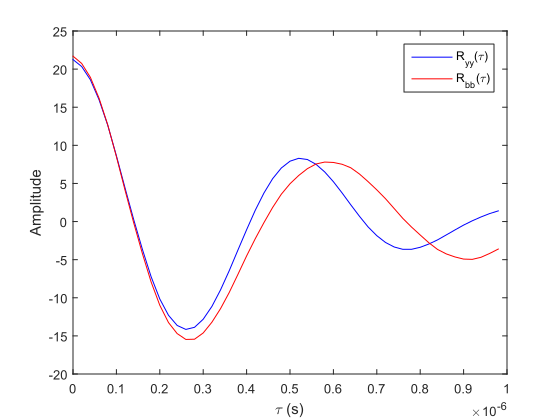
\includegraphics[scale=0.5]{autocorr.png}
    \label{autocorr}
    \caption{Comparaison des signaux réel et simulé par leur fonction d'autocorrélation}
\end{figure}

\begin{figure}[!h]
	\centering
	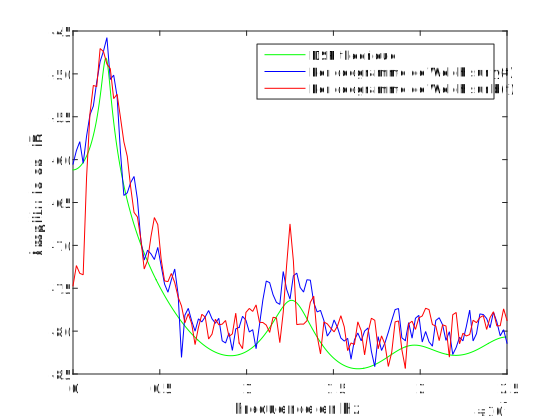
\includegraphics[scale=0.5]{dsp1.png}
    \label{dsp}
    \caption{Comparaison des signaux réel et simulé par leur contenu fréquentiel}
\end{figure}

\section{Optimisation du modèle par minimisation d'un critère test}

\subsection{critère d'Information d'Akaike}
\subsection{erreur de prédiction finale}

\begin{figure}[!h]
	\centering
	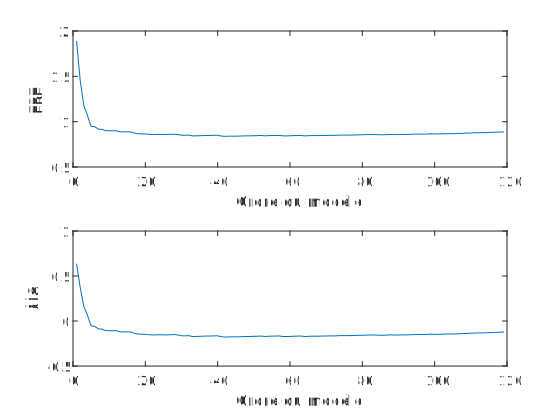
\includegraphics[scale=0.5]{criteres.png}
    \label{criteres}
    \caption{}
\end{figure}

\subsection{Comparaison de la DSP optimisée et non optimisée}

\begin{figure}[!h]
	\centering
	\includegraphics[scale=0.5]{otpi.png}
    \label{opti}
    \caption{Comparaison des signaux réel et simulé par leur contenu fréquentiel, avec optimisation de l'ordre du modèle.}
\end{figure}

\section{Conclusion}
Enjoy!

\end{document}